\documentclass{article}
\def\Rfunc#1{\textbf{#1()}}
\def\Rpkg#1{\textsl{#1}}
\def\Rarg#1{\textit{#1}}

\usepackage{fullpage}
\usepackage{times}
\usepackage{graphics}

\begin{document}

\section{Introduction}
Part of the movitation for this is to be able to deal
with cached computations, often in the context of dynamically
generated documents (Sweave and friends or XDynDocs),
or for interactive dynamic documents which are rendered
in R via an embedded browser widget.

An additional motivation is being able to summarize computations at a
high-level to aid understanding algorithms, scripts and the
computational process.  We want to view code at a higher level,
thinking more abstractly about the tasks rather than looking at the
details of the code.  This is, of course, where good software design
comes into play. But when writing scripts, software design is not
necessarily the focus of the author.  So we are enabling the author to
edit a script after it is created to annotate it at a higher level
with labels for the blocks.  We can also do this somewhat
programmatically, albeit imperfectly.

We are also advocating the notion of programmatically manipulating
scripts as objects that we can query and even modify and add code to.

\section{Scripts}
We are dealing with scripts, i.e. an ordered collection of R
expressions. These might be either individual expressions or blocks of
related code.  We introduce two classes: Script and AnnotatedScript.
Script is the general version; AnnotatedScript is a derived or
sub-class.  These are just lists of the expressions within the script.
A Script object also has its location, i.e. the file/URL from which it
was read.

Elements of a Script are of class ScriptNode.

There are several types of possible inputs for a script, i.e. formats
of source files.  We are considering simple R scripts, tangled code
extracted from an Sweave document, code extracted from an XML document
(i.e. Rdocbook from XDynDocs).  We also introduce the notion of an
``annotated R script'' which consists of code blocks each within
expression braces (i.e. { ... }) and labeled with elements of a
vocabulary that identify the high-level nature of the task that this
code is doing.  For example, initialization, dataInput, simulation,
EDA (exploratory data analysis), diagnostics, graphics, dataOutput.
These are intended to help the reader understand the high-level nature
of the code without focusing on the details of the actual expressions.
The task identifiers/labels  are added in the form
\begin{verbatim}
 initialization({
      library(codetools)
      library(CodeDepends)
 })
 plot(model({
     fit = lm(y ~ ., data)    
     plot(fit)
   }))
\end{verbatim}
One can even provide names for the elements of the script via
\begin{verbatim}
 mode.graphics = plot(model({
     fit = lm(y ~ ., data)    
     plot(fit)
   }))
\end{verbatim}
These can then be used to conveniently refer to a step
in the script, e.g. to run just that node, to run the code
up to that node, or to refer to a variable created within that
step.

\subsection{Reading Scripts}
Scripts are best read with the function \Rfunc{readScript}.  We can
specify the \Rarg{type} of the script or the function will attempt to guess
the type.
The possible types are ``xml'', ``R'', ``labeled'' and ``Stangled''.

We can specify the location as a file name, a connection (e.g. a URL)
or can specify the content of the script as a character vector via the
\Rarg{txt} parameter.



\section{ScriptNode Meta-Data}
getInputs is used to analyze a script or a node in a script
to compute the meta-information  about it, i.e
the input and output variables, the functions used, 
the files and libraries referenced.
\begin{verbatim}
f = system.file("samples", "namedAnnotatedScript.R", package = "CodeDepends")
sc = readScript(f, "labeled")
names(sc)
getInputs(sc)
getInputs(sc[[1]])
\end{verbatim}

Instead of using getInputs, we can use coercion as in
\begin{verbatim}
as(sc, "ScriptInfo")
\end{verbatim}

We can find the output/generated variables associated with the entire script
\begin{verbatim}
getVariables(sc)
\end{verbatim}


\section{Visualizing Relationships between Variables}
The meta-information allows us to determine which variables are inputs
to defining others (in terms of inputs and outputs to blocks).  We can
also visualize these via a graph with nodes displaying the variables
and edges illustrating which variables are inputs to others.  The
function \Rfunc{makeVariableGraph} is used for this. We can then plot this
using the \Rpkg{Rgraphviz} package.
\begin{verbatim}
f = system.file("samples", "results-multi.R", package = "CodeDepends")
g = makeVariableGraph(f)
library(Rgraphviz)
plot(g)
\end{verbatim}
\begin{figure}
  \centering
  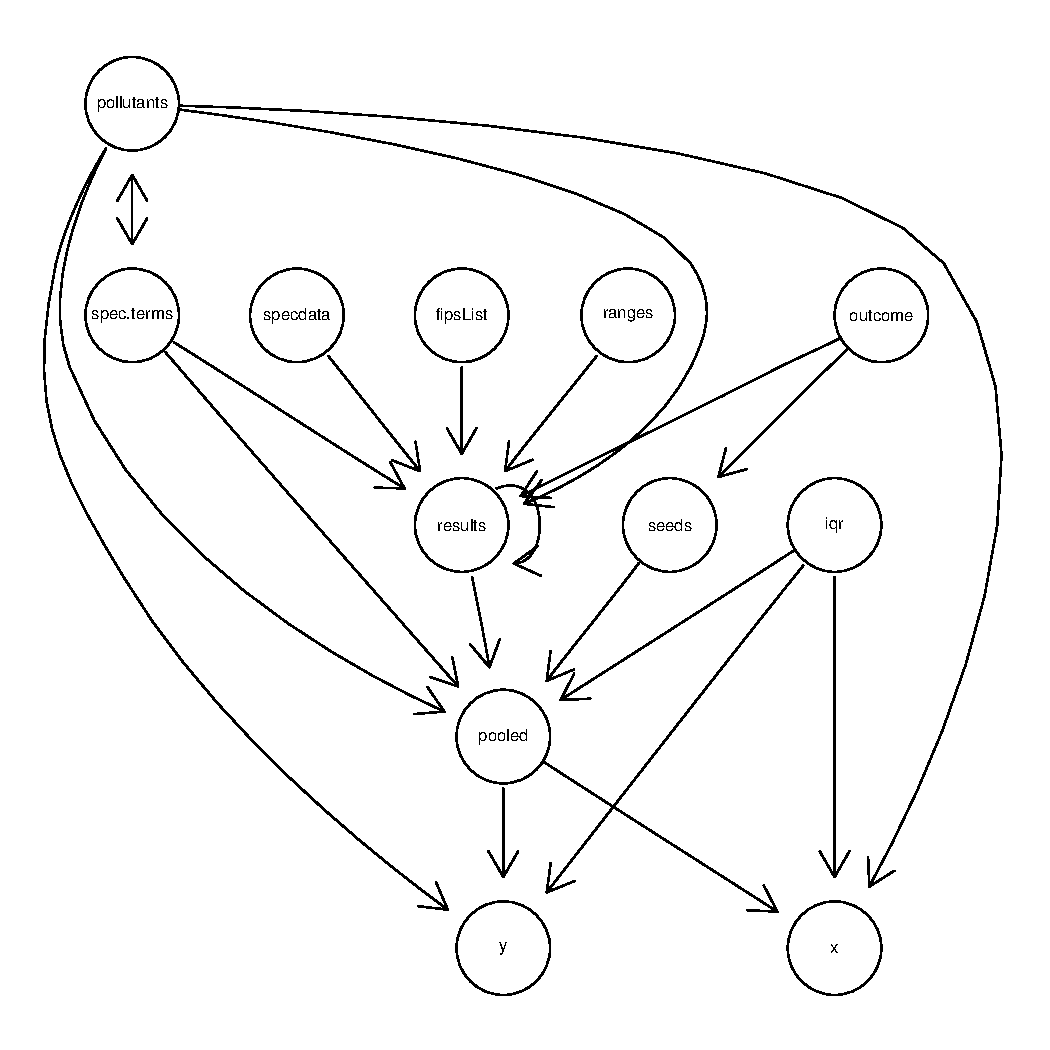
\includegraphics{variableGraph.pdf}
  \caption{Relationship between variables in \texttt{results-multi.R}}
\end{figure}

(Note that if you have previously computed the script, you can pass this
as the second argument to \Rfunc{makeVariableGraph}.)

\section{Visualizing Relationships between Tasks}
In addition to looking at individual variables, we
can visualize the relationships between tasks.
We can see how the outputs of one task are fed into 
other tasks. 
\begin{verbatim}
f = system.file("samples", "disjoint.R", package = "CodeDepends")
g = makeTaskGraph(f)
library(Rgraphviz)
plot(g)
\end{verbatim}
\begin{figure}
  \centering
  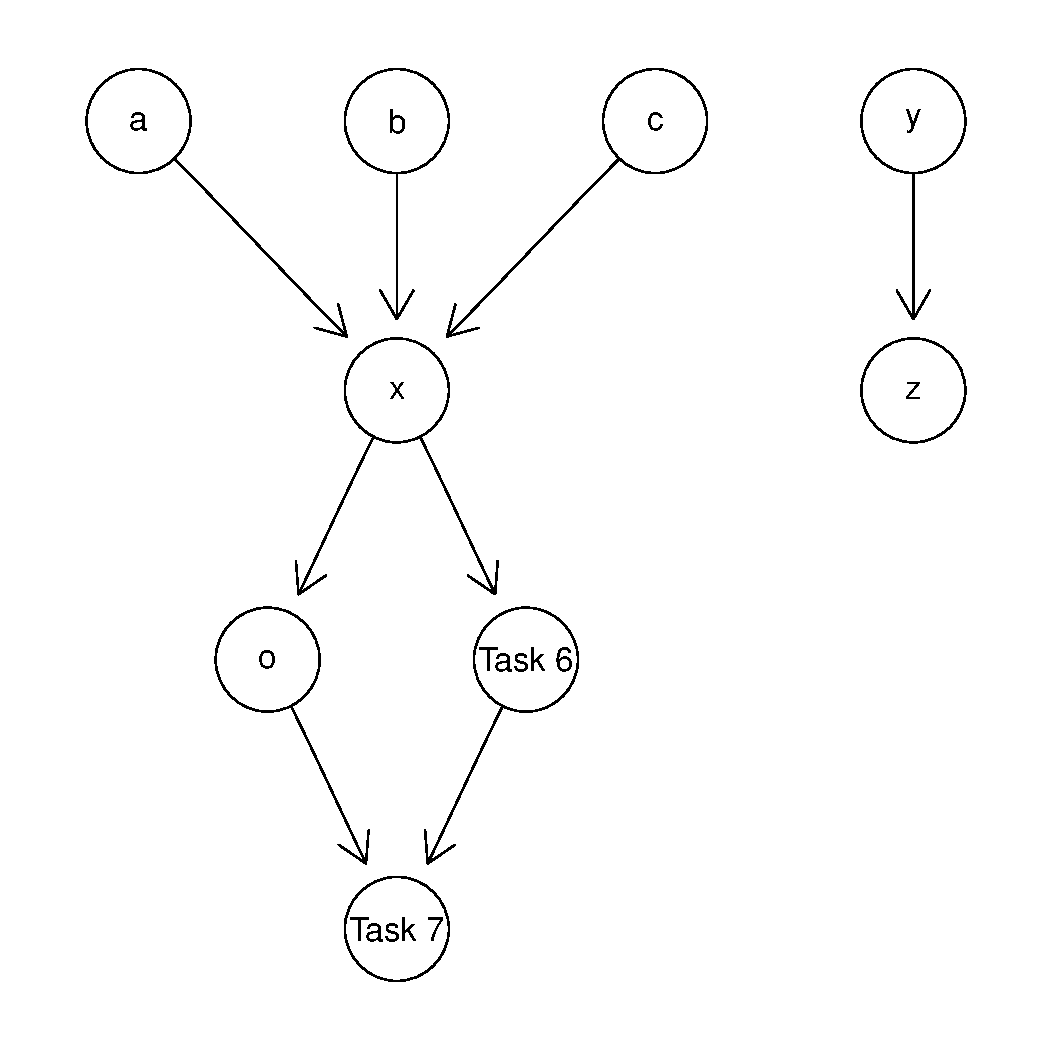
\includegraphics{taskGraph.pdf}
  \caption{Relationship between tasks in \texttt{disjoint.R}}
\end{figure}

When dealing with simple calls rather than 
code blocks containing multiple calls, the task graph
and the variable graph will be very similar.

We can use the SVGAnnotation to make this an interactive,
dynamic SVG plot.


\section{Variable Lifetimes and Garbage Collection}
When we call  functions, the intermediate or local variables
used by the function's body are garbage collected when the function
call is completed. In scripts, however, we often leave top-level intermediate
variables in the global environment even when they are no longer of
use in the remainder of the script.
With a little code analysis, for a given variable,
we can find the last expression in the script and 
add code to remove it and so allow the value to be garbage collected,
potentially freeing significant amounts of memory.

The function \Rfunc{findWhenUnneeded} determines the
index of the code block at which a variable is no longer used.
We can then add an expression to the end of this code block 
of the form
\begin{verbatim}
rm(varName)
\end{verbatim}

We can visualize the life cycles and the points at which 
the different variables are used and defined in the code
using \Rfunc{getDetailedTimelines}. This allows us to see if
variables should deleted or the order of the computations
changed to avoid holding variables in memory for long periods
over which they are not used.
An example is 
\begin{verbatim}
f = system.file("samples", "results-multi.R", package = "CodeDepends")
sc = readScript(f)
dtm = getDetailedTimelines(sc)
plot(dtm, main = "Variable time-line for results-multi.R")
\end{verbatim}
The result is
\begin{figure}
  \centering
  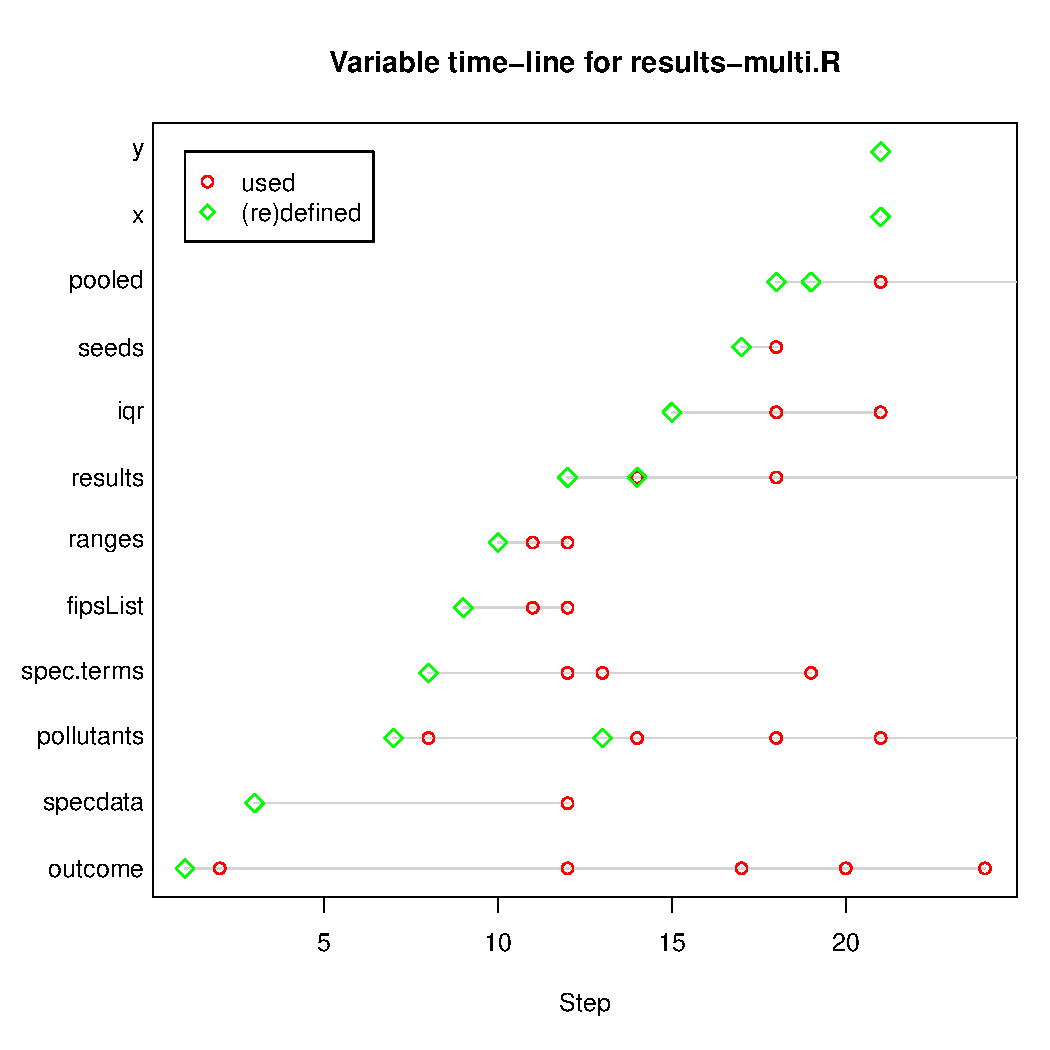
\includegraphics{resultsMultiTimeline.pdf}
  \caption{Time-line of variables in the \texttt{results-multi.R} script}
\end{figure}



\subsection{Functions}
We can also use the tools here for functions.
For example, let's find the ``length'' of
each function in the search path where ``length''
means the number of top-level expressions in the 
body.
\begin{verbatim}
z = sapply(search(), 
            function(x) {
             objs = objects(x)
             if(length(objs))
               structure(
                  sapply(objs, function(o) { 
                                tmp = get(o, x)
                                if(is.function(tmp)) 
                                   length(body(tmp)) 
                                else 
                                   0
                             }),
                  names = objs)
             else
                integer()
            })

names(z) = gsub("^package:", "", names(z))

sizes = data.frame(size = unlist(z), 
                   package = rep(names(z), sapply(z,length)))
\end{verbatim}
Let's visualize this data:
\begin{verbatim}
library(lattice)
densityplot(~size | package, sizes, plot.points = FALSE)
densityplot(~size, sizes, groups = package, 
             auto.key = list(columns = 5), plot.points = FALSE)
\end{verbatim}
We can then look at some of the big functions and summarize and visualize
these.
\begin{verbatim}
names(which.max(z[["utils"]]))
\end{verbatim}
yielding \Rfunc{read.DIF}.
Then we can look at the variables (including the function's parameters)
\begin{verbatim}
info = getInputs(read.DIF)
table(getVariables(info))
\end{verbatim}
and also create a graph
\begin{verbatim}
g = makeVariableGraph(info = info)
plot(g)
\end{verbatim}
Since we cannot use the annotation scheme for functions, 
it is useful to try to guess the tasks using
\Rfunc{guessTaskType} and to try to be able to 
group expressions into blocks.


\section{Function Call Graph}
This package allows us to compute 
the call graph between a set of functions.
We can specify a (named) list of functions
or a package or a single function (by name).
Methods then compute the call graph.
We can the visualize this using
\Rpkg{Rgraphviz}.
\begin{verbatim}
g = makeCallGraph("CodeDepends")
library(Rgraphviz)
plot(g, "circo")
\end{verbatim}
\begin{figure}
  \centering
  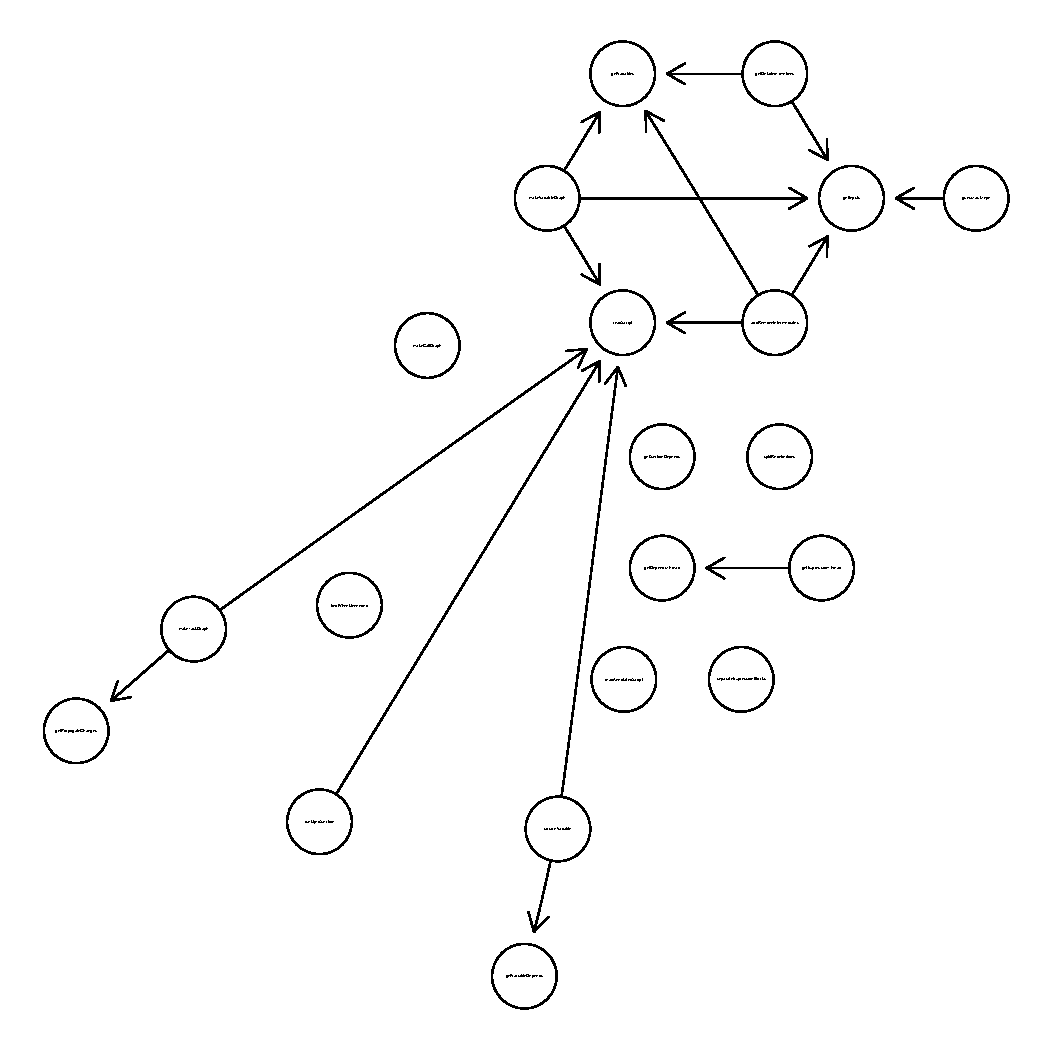
\includegraphics{callGraph.pdf}
  \caption{Function call graph for the CodeDepends package.}
\end{figure}


\section{Avoiding Redundant Computations}
Some scripts have redundant computations and being able to identify
these can save time and memory.  Clearly, computations that create
variables that are not used subsequently are typically not necessary.
(There may be side effects such as creating plots, files, opening
connections, etc.)  But, as in compilation, we might also identify
computations that are done several times that might be more
efficiently done once and assigned to an intermediate variable.

\section{Identifying Potential Parallelism}
Many scripts follow a strictly sequential path
where outputs from one block constitute the
inputs to the next block.
However, there are many which perform
one task and then another separate task and then
use the outputs from these two in the next task.
The fact that these two initial tasks are ``separate''
means they can be run in parallel.

\end{document}